\documentclass[11pt]{article}

% --------------------------------------------------
% Packages
% --------------------------------------------------
\usepackage[margin=1in]{geometry}
\usepackage{amsmath, amssymb, amsthm}
\usepackage{mathtools}
\usepackage{graphicx}
\usepackage{float}
\usepackage{enumitem}
\usepackage{hyperref}
\usepackage{xcolor}
\usepackage{tikz}
\usetikzlibrary{arrows.meta, positioning, calc}

% Pseudocode and algorithms
\usepackage{algorithm}
\usepackage{algpseudocode}

% Better fonts (optional)
\usepackage{lmodern}

% --------------------------------------------------
% Hyperref setup
% --------------------------------------------------
\hypersetup{
	colorlinks=true,
	linkcolor=blue,
	citecolor=blue,
	urlcolor=blue
}

% --------------------------------------------------
% Theorem-like environments
% --------------------------------------------------
\theoremstyle{definition}
\newtheorem{definition}{Definition}[section]
\newtheorem{theorem}{Theorem}[section]
\newtheorem{claim}{Claim}[section]
\newtheorem{remark}{Remark}[section]
\newtheorem{recall}{Recall}[section]

\theoremstyle{proof}
% Proof environment is built-in via amsthm

% --------------------------------------------------
% Custom commands
% --------------------------------------------------
\newcommand{\Gen}{\mathsf{Gen}}
\newcommand{\Enc}{\mathsf{Enc}}
\newcommand{\Dec}{\mathsf{Dec}}
\newcommand{\negl}{\mathsf{negl}}

% --------------------------------------------------
% Document
% --------------------------------------------------
\begin{document}
	
	\title{Public Key Crypto notes - 04}
	\author{By contributors}
	\date{March 3. 2026}
	\maketitle
	
	% --------------------------------------------------
	\section{Security of RSA}
	% --------------------------------------------------
	
	The security of RSA relies on the computational hardness of factoring large
	composite integers (compute $p, q$ from $N$).
	
	\subsection{The Factorization Problem}
	
	\begin{definition}[Factorization Experiment]
		\leavevmode
		Let $\mathsf{Factor}_A(n)$ be the following experiment:
		\begin{enumerate}
			\item Run $\Gen(1^n)$ to obtain an RSA modulus $N = pq$, where $p,q$ are primes.
			\item The adversary $A$ is given $N$ and outputs an integer $p'$.
			\item If $p' \mid N$ and $1 < p' < N$, then $\mathsf{Factor}_A(n) = 1$;
			otherwise, $\mathsf{Factor}_A(n) = 0$.
		\end{enumerate}
	\end{definition}
	
	\begin{definition}[Hardness of Factorization]
		The factorization problem is said to be \emph{hard} if for all probabilistic
		polynomial-time (PPT) adversaries $A$,
		$$
		\Pr[\mathsf{Factor}_A(n) = 1] \leq \negl(n).
		$$
	\end{definition}
	
	\begin{remark}
		In general, factorization is easy for random integers.
		For example, for a uniformly random integer $N$,
		$$
		\Pr[N \text{ is even}] = \tfrac{1}{2},
		$$
		in which case $p = 2$ is a trivial factor.
		However, when $N$ is generated as a product of two large primes
		$N = pq$, factorization is believed to be computationally hard.
	\end{remark}
	
	% --------------------------------------------------
	\subsection{Algorithms for Factorization}
	% --------------------------------------------------
	
	\subsubsection{Trial Division (Brute-force)}
	
	\begin{itemize}
		\item Try all integers $p = 2,3,\dots, \sqrt{N}$
		\item If some $p$ divides $N$, output $p$
	\end{itemize}
	
	\begin{remark}
		The running time of trial division is
		$$
		\mathcal{O}(\sqrt{N}) = \mathcal{O}(2^{n/2}),
		$$
		which is exponential in the bit-length $n$ of $N$.
	\end{remark}
	
	% --------------------------------------------------
	\subsubsection{Baby-Step Giant-Step Method for Factorization}
	% --------------------------------------------------
	
	Let $p,q$ be two primes of bit-length approximately $n$, i.e.,
	$$
	2^{n} \leq p,q < 2^{n+1},
	$$
	and let
	$$
	N = pq.
	$$
	
	Recall that Euler's totient function satisfies
	$$
	\varphi(N) = (p-1)(q-1) = pq - (p+q) + 1 = N - S + 1,
	$$
	where
	$$
	S = p + q.
	$$
	
	\begin{claim}
		Given $N$ and $S = p+q$, one can compute $p$ and $q$ in polynomial time.
	\end{claim}
	
	\begin{proof}
		Consider the quadratic polynomial
		$$
		f(x) = (x - p)(x - q).
		$$
		Expanding, we obtain
		$$
		f(x) = x^2 - (p+q)x + pq = x^2 - Sx + N.
		$$
		Thus, finding the roots of $f(x)$ yields $p$ and $q$.
		Since quadratic equations can be solved efficiently,
		$p$ and $q$ can be recovered in polynomial time given $N$ and $S$.
	\end{proof}
	
	\begin{remark}
		As $S$ has size $2^{n+2}$, we can write $m = [2^{\frac{n+2}{2}}]$ (the integer part of $m$) and write $S$ in the form:
		$$
		S = i \cdot m + j,
		$$
		where $0 \leq i,j \leq  m$.
		This idea underlies baby-step giant-step style approaches to factorization.
	\end{remark}
	
	% --------------------------------------------------
	\subsection{Baby-Step Giant-Step via Euler--Fermat}
	% --------------------------------------------------
	
	Recall Euler's theorem: for all $a$ such that $\gcd(a,N)=1$,
	$$
	a^{\varphi(N)} \equiv 1 \pmod N.
	$$
	
	Since $\varphi(N) = N - (p+q) + 1$, we obtain
	$$
	a^{N - S + 1} \equiv 1 \pmod N,
	$$
	where $S = p+q$.
	
	% --------------------------------------------------
	\subsubsection{Baby-Step Giant-Step Algorithm}
	% --------------------------------------------------
	
	\begin{itemize}
		\item Choose $x \in_R \mathbb{Z}_N^*$ uniformly at random.
		\item Fix a parameter $m$.
		\item Compute the following values:
	\end{itemize}
	
	$$
	x_i = (x^m)^i \quad \text{for } 0 \leq i \leq m
	$$
	
	$$
	x'_j = x^{N+1-j} \quad \text{for } 0 \leq j \leq m
	$$
	
	We look for a collision:
	$$
	x_i = x'_j \quad \text{for some } i,j.
	$$
	
	% --------------------------------------------------
	\subsubsection{Collision Illustration}
	% --------------------------------------------------
	
	\begin{figure}[H]
		\centering
		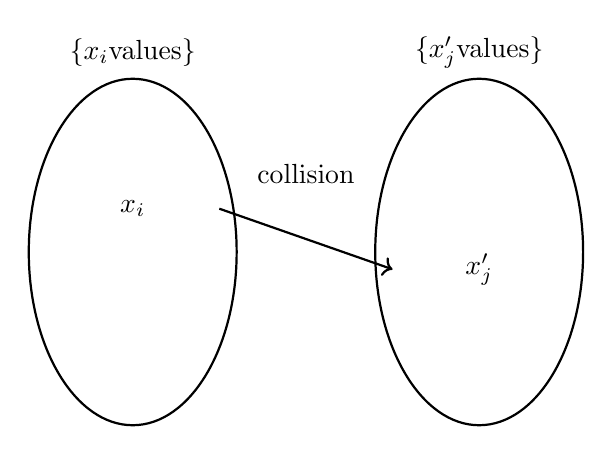
\begin{tikzpicture}[scale=1.1]
			
			% Left ellipse
			\draw[thick] (-2,0) ellipse (1.2 and 2);
			\node at (-2,2.3) {$\{x_i \text{values}\}$};
			\node at (-2,0.5) {$x_i$};
			
			% Right ellipse
			\draw[thick] (2,0) ellipse (1.2 and 2);
			\node at (2,2.3) {$\{x'_j \text{values}\}$};
			\node at (2,-0.2) {$x'_j$};
			
			% Arrow indicating collision
			\draw[->, thick] (-1,0.5) -- (1,-0.2);
			\node at (0,0.9) {collision};
			
		\end{tikzpicture}
		\caption{Baby-step giant-step collision: $x_i = x'_j$}
	\end{figure}
	
	% --------------------------------------------------
	\subsubsection{Extracting $S = p+q$}
	% --------------------------------------------------
	
	A collision implies:
	$$
	x^{i \cdot m} = x^i = x'_j = x^{N+1-j} \pmod N.
	$$
	
	Rewriting,
	$$
	x^{N+1-(i \cdot m + j)} \equiv 1 \pmod N.
	$$
	
	Thus,
	$$
	S = i \cdot m + j.
	$$
	
	% --------------------------------------------------
	\subsection{Remarks on the Method}
	% --------------------------------------------------
	
	\begin{remark}
		This is only a sketch.
		It may happen that
		$$
		x^a \equiv 1 \pmod N
		$$
		for some $a < \varphi(N)$.
		In that case, we only recover $S \bmod a$.
		However, the probability of this happening is not too large,
		and one can retry with a different choice of $x$.
		Even in such cases, partial information about $S$ may still be useful.
	\end{remark}
	
	\begin{remark}
		The time and space complexity of this approach is
		$$
		\mathcal{O}(m) = \mathcal{O}(2^{n/2}) = \mathcal{O}(\sqrt[4]{N}).
		$$
	\end{remark}
	
	\begin{remark}
		There exist algorithms such as Pollard's $\rho$ method
		with time complexity
		$$
		\mathcal{O}(\sqrt[4]{N})
		$$
		but only constant space complexity $\mathcal{O}(1)$.
	\end{remark}
	
	% --------------------------------------------------
	\subsection{Best Known Algorithms}
	% --------------------------------------------------
	
	\begin{remark}
		The best known general-purpose factorization algorithm is the
		\emph{General Number Field Sieve (GNFS)}, with running time
		$$
		\mathcal{O}(e ^{ (\sqrt[3]{\frac{64}{9}} + \epsilon) (\ln N)^\frac{1}{3} (\ln \ln N)^\frac{2}{3}})
		$$
	\end{remark}
	
	\begin{remark}[Key Size Implications]
		To achieve a security level comparable to AES-128,
		one needs an RSA modulus of size approximately
		$$
		N \approx 5000 \text{ bits}.
		$$
	\end{remark}
	
	% --------------------------------------------------
	\subsection{Choice of the Public Exponent}
	% --------------------------------------------------
	
	\begin{remark}[Choosing the Exponent $e$]
		If $e$ is very small, for example $e=3$, and the message $m$ is small,
		then interpreting $m$ as an integer we may have
		$$
		c = m^e < N.
		$$
		In this case, $m$ can be recovered directly by computing
		$$
		m = \sqrt[e]{c}.
		$$
	\end{remark}
	
	A standard choice for the public exponent is
	$$
	e = 2^{16} + 1 = 65537.
	$$
	
	This value is prime, and computing
	$$
	c = m^e \bmod N
	$$
	is efficient, since
	$$
	m^{2^{16}+1} = m \cdot m^{2^{16}}
	= m \cdot \bigl((m^2)^2 \cdots \bigr),
	$$
	which can be computed using repeated squaring (about $16$ squarings).
	
	% --------------------------------------------------
	\subsection{CPA Security of RSA}
	% --------------------------------------------------
	
	Recall the CPA (chosen-plaintext attack) experiment:
	
	\begin{enumerate}
		\item A key pair $(pk,sk)$ is generated.
		\item The adversary $A$ is given $pk$ and outputs two messages $m_0,m_1$.
		\item A random bit $b \in \{0,1\}$ is chosen and
		$$
		c = \Enc(pk,m_b)
		$$
		is computed.
		\item The adversary $A$ is given $c$ and outputs a guess $b'$ for $b$.
	\end{enumerate}
	
	\begin{remark}
		Textbook RSA is \emph{not} CPA-secure.
	\end{remark}
	
	Indeed, in step 4,
	$$
	c_0 = m_0^e \bmod N, \qquad
	c_1 = m_1^e \bmod N,
	$$
	and the adversary can simply output $b'$ such that
	$$
	c = c_b.
	$$
	
	\begin{remark}
		By randomizing the encryption, one can obtain CPA-secure encryption schemes.
	\end{remark}
	
	% --------------------------------------------------
	\subsection{Hard-Core Bits of RSA}
	% --------------------------------------------------
	
	\begin{theorem}
		Computing $x$ from $(N,e,x^e \bmod N)$ is as hard as computing
		the least significant bit $\mathrm{lsb}(x)$ of $x$.
	\end{theorem}
	
	That is, if there exists a PPT algorithm $A$ such that
	$$
	A(N,e,x^e \bmod N) = \mathrm{lsb}(x),
	$$
	then there exists a PPT algorithm $B$ such that
	$$
	B(N,e,x^e \bmod N) = x.
	$$
	
	\begin{remark}
		The bit $\mathrm{lsb}(x)$ is called a \emph{hard-core bit} of RSA.
	\end{remark}
	
	% --------------------------------------------------
	\subsection{Making RSA CPA-Secure}
	% --------------------------------------------------
	
	\begin{remark}
		One can construct a CPA-secure encryption scheme from RSA by encrypting
		a randomized message.
		Let
		$$
		m' = r \,\|\, m,
		$$
		where $r$ is chosen uniformly at random.
		The ciphertext is then computed as
		$$
		c = (m')^e \bmod N.
		$$
	\end{remark}

\end{document}
